% Options for packages loaded elsewhere
\PassOptionsToPackage{unicode}{hyperref}
\PassOptionsToPackage{hyphens}{url}
%
\documentclass[
]{book}
\usepackage{lmodern}
\usepackage{amssymb,amsmath}
\usepackage{ifxetex,ifluatex}
\ifnum 0\ifxetex 1\fi\ifluatex 1\fi=0 % if pdftex
  \usepackage[T1]{fontenc}
  \usepackage[utf8]{inputenc}
  \usepackage{textcomp} % provide euro and other symbols
\else % if luatex or xetex
  \usepackage{unicode-math}
  \defaultfontfeatures{Scale=MatchLowercase}
  \defaultfontfeatures[\rmfamily]{Ligatures=TeX,Scale=1}
\fi
% Use upquote if available, for straight quotes in verbatim environments
\IfFileExists{upquote.sty}{\usepackage{upquote}}{}
\IfFileExists{microtype.sty}{% use microtype if available
  \usepackage[]{microtype}
  \UseMicrotypeSet[protrusion]{basicmath} % disable protrusion for tt fonts
}{}
\makeatletter
\@ifundefined{KOMAClassName}{% if non-KOMA class
  \IfFileExists{parskip.sty}{%
    \usepackage{parskip}
  }{% else
    \setlength{\parindent}{0pt}
    \setlength{\parskip}{6pt plus 2pt minus 1pt}}
}{% if KOMA class
  \KOMAoptions{parskip=half}}
\makeatother
\usepackage{xcolor}
\IfFileExists{xurl.sty}{\usepackage{xurl}}{} % add URL line breaks if available
\IfFileExists{bookmark.sty}{\usepackage{bookmark}}{\usepackage{hyperref}}
\hypersetup{
  pdftitle={Documentação do projeto `Execução Orçamentária e Financeira do Governo Federal' (``Projeto Caixa'')},
  pdfauthor={R6 Estatística e Treinamentos LTDA},
  hidelinks,
  pdfcreator={LaTeX via pandoc}}
\urlstyle{same} % disable monospaced font for URLs
\usepackage{longtable,booktabs}
% Correct order of tables after \paragraph or \subparagraph
\usepackage{etoolbox}
\makeatletter
\patchcmd\longtable{\par}{\if@noskipsec\mbox{}\fi\par}{}{}
\makeatother
% Allow footnotes in longtable head/foot
\IfFileExists{footnotehyper.sty}{\usepackage{footnotehyper}}{\usepackage{footnote}}
\makesavenoteenv{longtable}
\usepackage{graphicx,grffile}
\makeatletter
\def\maxwidth{\ifdim\Gin@nat@width>\linewidth\linewidth\else\Gin@nat@width\fi}
\def\maxheight{\ifdim\Gin@nat@height>\textheight\textheight\else\Gin@nat@height\fi}
\makeatother
% Scale images if necessary, so that they will not overflow the page
% margins by default, and it is still possible to overwrite the defaults
% using explicit options in \includegraphics[width, height, ...]{}
\setkeys{Gin}{width=\maxwidth,height=\maxheight,keepaspectratio}
% Set default figure placement to htbp
\makeatletter
\def\fps@figure{htbp}
\makeatother
\setlength{\emergencystretch}{3em} % prevent overfull lines
\providecommand{\tightlist}{%
  \setlength{\itemsep}{0pt}\setlength{\parskip}{0pt}}
\setcounter{secnumdepth}{5}
\usepackage{booktabs}
\usepackage[utf8]{inputenc}
\usepackage{amsthm}
\makeatletter
\def\thm@space@setup{%
  \thm@preskip=8pt plus 2pt minus 4pt
  \thm@postskip=\thm@preskip
}
\makeatother
\AtBeginDocument{\renewcommand{\chaptername}{Capítulo}}
\usepackage[]{natbib}
\bibliographystyle{apalike}

\title{Documentação do projeto `Execução Orçamentária e Financeira do Governo Federal' (``Projeto Caixa'')}
\author{R6 Estatística e Treinamentos LTDA}
\date{2020-02-20}

\begin{document}
\frontmatter
\maketitle

{
\setcounter{tocdepth}{1}
\tableofcontents
}
\mainmatter
\hypertarget{introduuxe7uxe3o}{%
\chapter{Introdução}\label{introduuxe7uxe3o}}

O objetivo deste projeto é analisar o comportamento do caixa e das obrigações financeiras dos órgãos federais, com a finalidade de fornecer informações para a gestão da programação financeira por parte do Tesouro Nacional, além de identificar oportunidades de melhorias nesse processo, e possivelmente fundamentar a criação de indicadores para avaliação da gestão financeira das unidades do Governo Federal.

Elencamos aqui alguns aspectos importantes do projeto.

\hypertarget{questuxf5es-investigadas}{%
\section{Questões investigadas}\label{questuxf5es-investigadas}}

De início, analisamos o perfil das despesas e receitas das unidades do Governo Federal, começando com os órgãos do Ministério da Justiça (que já possui um sistema de acompanhamento de despesas bem estruturado).

A análise procurou compatibilizar as informações orçamentárias com as informações financeiras. Chamamos de \emph{classificadores orçamentários}: Função, Subfunção, Programa, Ação, Grupo de Despesa, Modalidade de Aplicação, Elemento de Despesa, Indicador de Resultado EOF, Indicador de Exceção Decreto. Como \emph{classificadores financeiros}, nos referimos, essencialmente, à Vinculação de Pagamento.

A \emph{Fonte de Recurso} é um classificador comum a esses dois contextos, orçamentário e financeiro.

Com esse escopo em mente, em parceria com a equipe do GT-CEAD, as seguintes questões foram abordadas neste projeto:

\begin{enumerate}
\def\labelenumi{\alph{enumi}.}
\item
  Qual o comportamento do caixa e das obrigações a pagar (e da disponibilidade líquida) no período analisado\footnote{Por órgão, por unidade e por fonte de recursos.}?
\item
  Existem casos em que unidades de um mesmo órgão permanecem com disponibilidade líquida negativa, enquanto outras unidades desse mesmo órgão encontram-se com disponibilidade positiva? E se considerar a fonte de recursos, há casos em que o órgão passa por períodos com disponibilidade negativa em uma fonte enquanto há recursos disponíveis em outra fonte? E se considerar as duas situações conjuntamente\footnote{Ou seja, uma unidade de um mesmo órgão fica com disponibilidade negativa em uma fonte, enquanto outra unidade desse mesmo órgão possui disponibilidade positiva nessa mesma fonte.}?
\item
  Como as classificações orçamentárias se relacionam com as classificações financeiras? Especificamente, é possível identificar certos tipos de despesas que são sempre (ou frequentemente) pagas com recursos de determinadas vinculações?
\item
  Caso seja possível a identificação mencionada em (c), as questões (a) e (b) seriam revisitadas para estimar a disponibilidade líquida para cada vinculação, considerando as classificações orçamentárias das obrigações. Nesse cenário, existem unidades com saldo total suficiente para cobrir todas as suas obrigações, porém com insuficiência em algumas vinculações?
\item
  Qual o comportamento do caixa das unidades em termos de movimentações?
\item
  Qual o intervalo entre duas operações\footnote{Uma despesa alta seguida de um recebimento de recursos também alto.} de grande porte?
\end{enumerate}

Para responder essas perguntas, utilizamos ferramentas descritivas e de modelagem preditiva, descritas nos Capítulos 3 e 4, respectivamente.

\hypertarget{as-bases-de-dados}{%
\section{As bases de dados}\label{as-bases-de-dados}}

Para responder as questões levantadas no item anterior, os dados do SIAFI foram divididos em três bases de dados:

\begin{itemize}
\item
  \begin{enumerate}
  \def\labelenumi{\arabic{enumi}.}
  \tightlist
  \item
    base de movimentações diárias do limite de saque;
  \end{enumerate}
\item
  \begin{enumerate}
  \def\labelenumi{\arabic{enumi}.}
  \setcounter{enumi}{1}
  \tightlist
  \item
    base de pagamentos diários;
  \end{enumerate}
\item
  \begin{enumerate}
  \def\labelenumi{\arabic{enumi}.}
  \setcounter{enumi}{2}
  \tightlist
  \item
    base de movimentações diárias nas obrigações a pagar.
  \end{enumerate}
\end{itemize}

Com as Tabelas 1 e 3, calculamos a \emph{disponibilidade líquida diária} a partir da subtração entre os saldos diários do caixa (Tabela 1) e as obrigações a pagar (Tabela 3), para cada unidade gestora ou órgão, e para cada fonte de recursos.

Com as Tabelas 1 e 2, relacionamos no contexto dos pagamentos, as informações orçamentrárias (Tabela 2) com os vínculos de pagamento (Tabela 1).

Finalmente com a Tabela 1, analisamos as movimentações para tipo de documento, obtendo um histórico das movimentações de cada órgão e cada Unidade Gestora.

Na primeira etapa do projeto, essas bases foram estudadas e validadas. Bases auxiliares também foram construídas para facilitar as análises subsequentes. A documentação dessa etapa se encontra no Capítulo 2.

\hypertarget{anuxe1lise-descritiva}{%
\section{Análise descritiva}\label{anuxe1lise-descritiva}}

Dada a riqueza de informações e granularidade das bases de dados, todos os resultados descritivos foram construídos em uma aplicação online, que permite a manipulação das visualizações a partir de filtros e seletores.

O aplicativo pode ser acessado a partir do seguinte link: \url{https://rseis.shinyapps.io/explorador_disponibilidades_liquidas_v2/}

O código-fonte e manutenção do aplicativo foram repassados à equipe do GT-CEAD ao fim do projeto.

Um resumo dos principais resultados se encontra no Capítulo 3.

\hypertarget{anuxe1lise-preditiva}{%
\section{Análise preditiva}\label{anuxe1lise-preditiva}}

Os modelos utilizados neste projeto consideraram os métodos em estado da arte dentro do contexto de modelagem preditiva, como florestas aleatórias, o algorítmo XGBoost e redes neurais.

A descrição dos modelos ajustados e seus resultados se encontram no Capítulo 4.

\hypertarget{oficina-de-repasses-e-implementauxe7uxe3o-dos-produtos}{%
\section{Oficina de repasses e implementação dos produtos}\label{oficina-de-repasses-e-implementauxe7uxe3o-dos-produtos}}

A última etapa do projeto consistiu de uma oficina de repasses, realizada presencialmente no GT-CEAD, no Tesouro Nacional, em Brasília. Nessa oficina, foi discutida a teoria por trás dos métodos aplicados, tal como apresentada neste relatório. Também foram apresentados e explicados os scripts em linguagem de programação R utilizados para implementar os modelos.

\hypertarget{validauxe7uxe3o-e-compreensuxe3o-dos-dados}{%
\chapter{Validação e Compreensão dos Dados}\label{validauxe7uxe3o-e-compreensuxe3o-dos-dados}}

\hypertarget{introduuxe7uxe3o-1}{%
\section{Introdução}\label{introduuxe7uxe3o-1}}

A base de dados do SIAFI concentra as informações geradas pelo processo de execução orçamentária e programação financeira do Governo Federal. Este projeto tem como objetivo gerar conhecimento sobre o comportamento do caixa e das obrigações financeiras dos órgãos federais para fins de gestão da programação financeira por parte do Tesouro Nacional, além de identificar oportunidades de melhorias nesse processo e, possivelmente, fundamentar a criação de indicadores para avaliação da gestão financeira das unidades do Governo Federal.

Este é o primeiro dos quatro relatórios que irão compor o projeto e descreve o processo de conhecimento, ajuste e preparo das bases de dados para análises subsequentes.

\hypertarget{questuxf5es-elementares}{%
\section{Questões elementares}\label{questuxf5es-elementares}}

Para nortear as análises das próximas etapas, nessa primeira fase de conhecimento do problema e da base, foram levantadas as seguintes questões:

\begin{enumerate}
\def\labelenumi{\alph{enumi}.}
\item
  Qual o comportamento do caixa e das obrigações a pagar (e da disponibilidade líquida) no período analisado\footnote{Por órgão, por unidade e por fonte de recursos.}?
\item
  Existem casos em que unidades de um mesmo órgão permanecem com disponibilidade líquida negativa, enquanto outras unidades desse mesmo órgão encontram-se com disponibilidade positiva? E se considerar a fonte de recursos, há casos em que o órgão passa por períodos com disponibilidade negativa em uma fonte enquanto há recursos disponíveis em outra fonte? E se considerar as duas situações conjuntamente\footnote{Ou seja, uma unidade de um mesmo órgão fica com disponibilidade negativa em uma fonte, enquanto outra unidade desse mesmo órgão possui disponibilidade positiva nessa mesma fonte.}?
\item
  Como as classificações orçamentárias se relacionam com as classificações financeiras? Especificamente, é possível identificar certos tipos de despesas que são sempre (ou frequentemente) pagas com recursos de determinadas vinculações?
\item
  Caso seja possível a identificação mencionada em (c), as questões (a) e (b) seriam revisitadas para estimar a disponibilidade líquida para cada vinculação, considerando as classificações orçamentárias das obrigações. Nesse cenário, existem unidades com saldo total suficiente para cobrir todas as suas obrigações, porém com insuficiência em algumas vinculações?
\item
  Qual o comportamento do caixa das unidades em termos de movimentações?
\item
  Qual o intervalo entre duas operações\footnote{Uma despesa alta seguida de um recebimento de recursos também alto.} de grande porte?
\end{enumerate}

\hypertarget{bases-de-dados-levantadas-para-endereuxe7ar-as-questuxf5es}{%
\section{Bases de dados levantadas para endereçar as questões}\label{bases-de-dados-levantadas-para-endereuxe7ar-as-questuxf5es}}

O perfil das despesas do \textbf{Ministério da Justiça} será utilizado como ponto de partida das análises descritivas e exploratórias. A escolha deste órgão foi em virtude do seu excelente sistema de acompanhamento das despesas.

Ao todo, três bases foram extraídas:

\begin{itemize}
\tightlist
\item
  \texttt{lim\_saque} com as movimentações de limites de saque;
\item
  \texttt{obrigacoes} com as movimentações de obrigações a pagar; e
\item
  \texttt{pagamentos} com as movimentações de pagamentos;
\end{itemize}

A partir destas, outras três tabelas derivadas foram construídas. As descrições detalhadas estão na seção seguinte.

\begin{itemize}
\item
  \texttt{disponibilidades\_liquidas\_diarias} com as informações diárias de \textbf{saldo disponível} e \textbf{obrigações a pagar} de cada UG para cada fonte de recursos;
\item
  \texttt{vinculacao\_de\_pagamentos} com informações diárias pareadas de \textbf{pagamentos}, \textbf{saldo disponível} e \textbf{vinculações de pagamentos} de cada documento;
\item
  \texttt{lim\_saque\_por\_tipo\_de\_documento} com as informações diárias de \textbf{saldo disponível} por tipo de documento (e.g.~NS, OB, PF, etc.).
\end{itemize}

Verificou-se que as extrações \textbf{encontram-se prontas para análise} e com replicações em formatos \texttt{.rds} para serem leitas pelo software R. Abaixo estão listados os seus respectivos campos.

\hypertarget{base-1-movimentauxe7uxf5es-diuxe1rias-do-limite-de-saque}{%
\section{Base 1: Movimentações diárias do Limite de Saque}\label{base-1-movimentauxe7uxf5es-diuxe1rias-do-limite-de-saque}}

\textbf{Filtro:} item de informação ``LIMITES DE SAQUE''.

\textbf{Campos:}

\begin{itemize}
\tightlist
\item
  Órgão Máximo
\item
  Órgão
\item
  UG
\item
  \textbf{Vinculação de Pagamento}
\item
  Fonte de Recursos Detalhada
\item
  Fonte de Recursos
\item
  Documento Lançamento
\item
  Movimento / Valor Financeiro
\end{itemize}

\hypertarget{base-2-pagamentos-diuxe1rios}{%
\section{Base 2: Pagamentos diários}\label{base-2-pagamentos-diuxe1rios}}

\textbf{Filtro:} item de informação ``PAGAMENTOS TOTAIS''.

\textbf{Campos:}

\begin{itemize}
\tightlist
\item
  Órgão Máximo
\item
  Órgão
\item
  UG
\item
  Fonte de Recursos Detalhada
\item
  Fonte de Recursos
\item
  \textbf{Função}
\item
  \textbf{Subfunção}
\item
  \textbf{Programa}
\item
  \textbf{Ação}
\item
  \textbf{Grupo de Despesa}
\item
  \textbf{Modalidade de Aplicação}
\item
  \textbf{Elemento de Despesa}
\item
  \textbf{Indicador de Resultado EOF} (indica se a despesa é primária ou financeira, entre outras coisas)
\item
  \textbf{Indicador de Exceção Decreto}
\item
  \textbf{Ano do Empenho}
\item
  \textbf{Empenho}
\item
  \textbf{Órgão Máximo da UO}
\item
  Documento Lançamento
\item
  Movimento / Valor Financeiro
\end{itemize}

\hypertarget{base-3-movimentauxe7uxf5es-diuxe1rias-em-obrigauxe7uxf5es-a-pagar}{%
\section{Base 3: Movimentações diárias em obrigações a pagar}\label{base-3-movimentauxe7uxf5es-diuxe1rias-em-obrigauxe7uxf5es-a-pagar}}

\textbf{Filtro:} item de informação ``VALORES LIQUIDADOS A PAGAR (EXERCICIO + RP)''.

\textbf{Campos:}

\begin{itemize}
\tightlist
\item
  Órgão Máximo
\item
  Órgão
\item
  UG
\item
  Fonte Detalhada
\item
  Fonte (posições 3 e 4 da fonte detalhada -- exemplo: se a fonte detalhada é: \texttt{0100123456}, a fonte será \texttt{00})
\item
  \textbf{Função}
\item
  \textbf{Subfunção}
\item
  \textbf{Programa}
\item
  \textbf{Ação}
\item
  \textbf{Grupo de Despesa}
\item
  \textbf{Modalidade de Aplicação}
\item
  \textbf{Elemento de Despesa}
\item
  \textbf{Indicador de Resultado EOF} (indica se a despesa é primária ou financeira, entre outras coisas)
\item
  \textbf{Indicador de Exceção Decreto}
\item
  \textbf{Ano do Empenho}
\item
  \textbf{Empenho}
\item
  \textbf{Órgão Máximo da UO}
\item
  Movimento / Valor Financeiro
\end{itemize}

\hypertarget{tabelas-derivadas}{%
\section{Tabelas Derivadas}\label{tabelas-derivadas}}

\hypertarget{disponibilidades-luxedquidas-diuxe1rias}{%
\subsection{Disponibilidades líquidas Diárias}\label{disponibilidades-luxedquidas-diuxe1rias}}

\begin{itemize}
\item
  Informações diárias de \textbf{saldo disponível} e \textbf{obrigações a pagar} de cada UG para cada fonte de recursos.
\item
  Útil para as questões \textbf{a}, \textbf{c} e \textbf{e}.
\item
  Cruzamento entre as bases \texttt{lim\_saque} e \texttt{obrigacoes} pelas chaves \texttt{NO\_DIA\_COMPLETO}, \texttt{NO\_FONTE\_RECURSO} e \texttt{NO\_UG}.
\item
  Observações: 352.037
\item
  Campos: 11
\end{itemize}

\begin{verbatim}
* NO_DIA_COMPLETO         `<date> 2017-08-22, 2017-08-23, 2017-08-24, 2017-08…`
* NO_UG                   `<chr> "ACADEMIA NACIONAL DA POLICIA RODOV. FEDERAL…`
* NO_ORGAO                `<chr> "DEPARTAMENTO DE POLICIA RODOVIARIA FEDERAL/…`
* NO_FONTE_RECURSO        `<chr> "RECEITAS DE CONCURSOS DE PROGNOSTICOS", "RE…`
* saldo_diario            `<dbl> -2779.98, -5654.96, -7356.26, -5601.60, -560…`
* obrigacoes_a_pagar      `<dbl> 0.000000e+00, 0.000000e+00, 0.000000e+00, 0.…`
* disponibilidade_liquida `<dbl> -2779.98, -5654.96, -7356.26, -5601.60, -560…`
* ano                     `<dbl> 2017, 2017, 2017, 2017, 2017, 2017, 2017, 20…`
* mes                     `<dbl> 8, 8, 8, 8, 8, 8, 8, 8, 8, 8, 9, 9, 9, 9, 9,…`
* dia                     `<int> 22, 23, 24, 25, 26, 27, 28, 29, 30, 31, 1, 2…`
* paded                   `<lgl> TRUE, TRUE, TRUE, TRUE, FALSE, FALSE, TRUE, …`
\end{verbatim}

\hypertarget{vinculauxe7uxe3o-de-pagamentos}{%
\subsection{Vinculação de Pagamentos}\label{vinculauxe7uxe3o-de-pagamentos}}

\begin{itemize}
\item
  Informações diárias pareadas de \textbf{pagamentos}, \textbf{saldo disponível} e \textbf{vinculações de pagamentos} de cada documento.
\item
  Útil para as questões \textbf{b}, \textbf{c} e \textbf{e}.
\item
  Cruzamento entre as bases \texttt{lim\_saque} e \texttt{pagamentos} pelas chaves \texttt{NO\_DIA\_COMPLETO} e \texttt{ID\_DOCUMENTO}.
\item
  Observações: 1.005.187
\item
  Campos: 7
\end{itemize}

\begin{verbatim}
* NO_DIA_COMPLETO         `<chr> "01/02/2017", "01/02/2017", "01/02/2017", "0…`
* ID_DOCUMENTO            `<chr> "194003192082017OB800016", "194003192082017O…`
* pagamento               `<dbl> 20.79, 724.21, 8000.00, 76.95, -15188.99, -9…`
* NO_VINCULACAO_PAGAMENTO `<chr> "CUSTEIO/INVESTIMENTO - RESUL.PRIM = 2", "CU…`
* vinculacoes_distintas   `<int> 1, 1, 1, 1, 1, 1, 1, 1, 1, 1, 1, 1, 1, 1, 1,…`
* saldo_diario            `<dbl> -20.79, -724.21, -8000.00, -76.95, 15188.99,…`
* pagamento_por_saldo     `<dbl> -1, -1, -1, -1, -1, -1, -1, -1, -1, -1, -1, …`
\end{verbatim}

\hypertarget{limimtes-de-saque-por-tipo-de-documento}{%
\subsection{Limimtes de Saque Por Tipo De Documento}\label{limimtes-de-saque-por-tipo-de-documento}}

\begin{itemize}
\item
  Informações diárias de \textbf{saldo disponível} por tipo de documento. Os tipos de documentos são: \texttt{DF}, \texttt{DR}, \texttt{GF}, \texttt{GP}, \texttt{GR}, \texttt{NL}, \texttt{NS}, \texttt{OB}, \texttt{PF} e \texttt{RA}.
\item
  Útil para a questão \textbf{d}.
\item
  Derivada da base \texttt{lim\_saque}.
\item
  Observações: 254.667
\item
  Campos: 7
\end{itemize}

\begin{verbatim}
* tipo_de_documento  `<chr> "DF", "DF", "DF", "DF", "DF", "DF", "DF", "DF", "…`
* NO_DIA_COMPLETO    `<chr> "01/02/2017", "01/02/2017", "01/02/2017", "01/02/…`
* NO_UG              `<chr> "COORD. REG. NOROESTE DO MATO GROSSO/MT", "COORDE…`
* NO_ORGAO           `<chr> "FUNDACAO NACIONAL DO INDIO", "DEPARTAMENTO DE PO…`
* NO_ITEM_INFORMACAO `<chr> "LIMITES DE SAQUE (OFSS, DIVIDA, BACEN E PREV)", …`
* NO_FONTE_RECURSO   `<chr> "RECURSOS ORDINARIOS", "RECURSOS ORDINARIOS", "TX…`
* saldo_diario       `<dbl> -35.47, -2089.65, -3644.19, -12.01, -14.94, -31.3…`
\end{verbatim}

\hypertarget{disponibilidades-luxedquidas}{%
\chapter{Disponibilidades Líquidas}\label{disponibilidades-luxedquidas}}

Para responder a questão (a){[}a. Qual o comportamento do caixa e das obrigações a pagar (e da disponibilidade líquida) no período analisado?{]} sobre disponibilidades líquidas das UGs e as respectivas fontes de recursos, elaboramos os seguintes indicadores:

\begin{itemize}
\item
  \textbf{Indicador de acumulação de disponibilidade líquida:} acusa potencial problema de UGs que estariam recebendo recursos de fontes que já apresentava valores acumulados.
\item
  \textbf{Indicador de persistência de saldo positivo:} acusa potencial problema de recurso estacionado por longo período.
\end{itemize}

Anexo ao relatório, a tabela \textbf{``indicadores.csv''} contém a lista de todas as UGs e fontes de recursos e seus respectivos valores dos indicadores.

\hypertarget{indicador-de-acumulauxe7uxe3o-de-disponibilidade-luxedquida-i_adl}{%
\section{\texorpdfstring{Indicador de acumulação de disponibilidade líquida (\(I_{ADL}\))}{Indicador de acumulação de disponibilidade líquida (I\_\{ADL\})}}\label{indicador-de-acumulauxe7uxe3o-de-disponibilidade-luxedquida-i_adl}}

Indicador que apresenta valor alto quando uma UG apresenta disponibilidade líquida que apenas cresce com o passar do tempo para uma determinada fonte de recurso.

\hypertarget{definiuxe7uxe3o}{%
\subsection{Definição}\label{definiuxe7uxe3o}}

Seja \(y_i\) a disponibilidade líquida no dia \(i\),

\(I_{ADL} = P_1 + P_2\)

em que

\[
P_1 = \frac{1}{N}\sum I(y_i > y_{i - 1})
\]

e \textbf{para quando a disponibilidade diminui}

\[
P_2 = \frac{1}{N_{y_i < y_{i - 1}}}\sum I(|y_i -y_{i - 1}| < \sigma)
\]

Em outras palavras, o indicador aponta curvas crescentes (\(P_1\)) permitindo pequenas perturbações (\(P_2\)).

\hypertarget{exemplos}{%
\subsection{Exemplos}\label{exemplos}}

Abaixo estão as três curvas com os maiores valores de \(I_{ADL}\):

\begin{tabular}{l|l|l|r}
\hline
Órgão & Fonte de Recursos & UG & IADL\\
\hline
CONSELHO ADMINISTRATIVO DE DEFESA ECONOMICA & RECURSOS NAO-FINANCEIROS DIRETAM. ARRECADADOS & CONSELHO ADMINISTRATIVO DE DEFESA ECONOMICA & 1.26\\
\hline
FUNDO NACIONAL ANTIDROGAS & RECURSOS NAO-FINANCEIROS DIRETAM. ARRECADADOS & FUNDO NACIONAL ANTIDROGAS & 1.21\\
\hline
DEPARTAMENTO DE POLICIA RODOVIARIA FEDERAL/MJ & RECURSOS DIVERSOS & SUPERINTENDENCIA REG. POL. RODV. FEDERAL-BA & 1.15\\
\hline
\end{tabular}

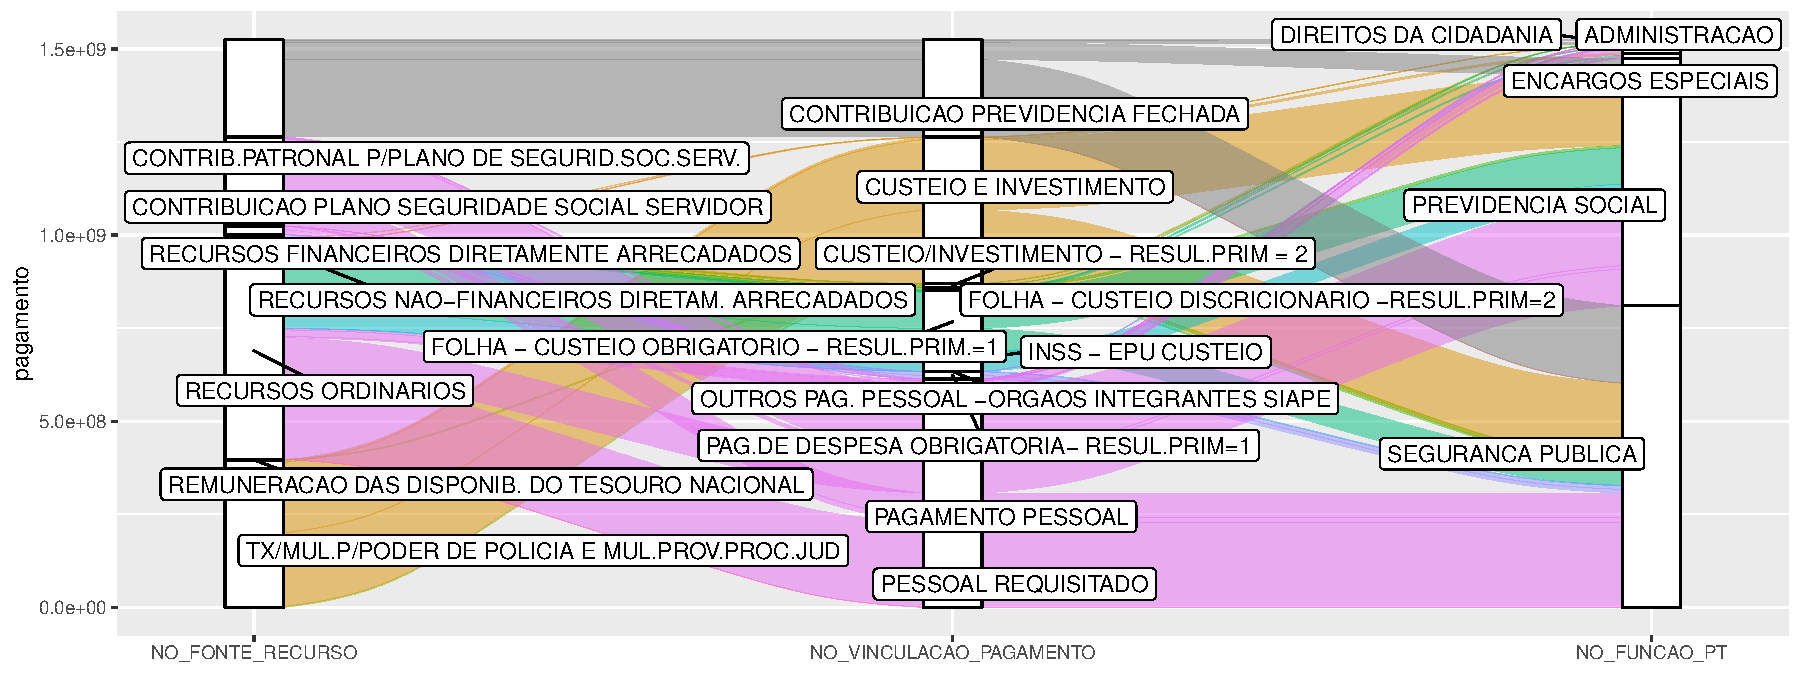
\includegraphics{03-quadro-historico_files/figure-latex/unnamed-chunk-4-1.pdf}

\hypertarget{indicador-de-persistuxeancia-de-saldo-positivo-i_psp}{%
\section{\texorpdfstring{Indicador de persistência de saldo positivo (\(I_{PSP}\))}{Indicador de persistência de saldo positivo (I\_\{PSP\})}}\label{indicador-de-persistuxeancia-de-saldo-positivo-i_psp}}

Indicador com valores altos para as curvas que apresentarem saldos positivos por longa duração de tempo no acumulado do período analisado.

\hypertarget{definiuxe7uxe3o-1}{%
\subsection{Definição}\label{definiuxe7uxe3o-1}}

Área sob a curva de disponibilidade líquida ponderada pela soma de todas as obrigações pagas.

Seja \(y_i\) a disponibilidade líquida no dia \(i\) e \(o_i\) as obrigações pagas no dia \(i\),

\[
I_{PSP} = \frac{\sum y_i}{\sum o_i}
\]

\hypertarget{exemplos-1}{%
\subsection{Exemplos}\label{exemplos-1}}

Abaixo estão as três curvas com os maiores valores de \(I_{PSP}\):

\begin{tabular}{l|l|l|r}
\hline
Órgão & Fonte de Recursos & UG & IPSP\\
\hline
MINISTERIO DA JUSTICA E SEGURANCA PUBLICA & RECURSOS ORDINARIOS & COORDENACAO-GERAL DE ORCAMENTO E FINANCAS-MJ & 0.48\\
\hline
DEPARTAMENTO DE POLICIA FEDERAL & RECURSOS NAO-FINANCEIROS DIRETAM. ARRECADADOS & COORDENACAO DE ORCAMENTO E FINANCAS - COF/DPF & 0.93\\
\hline
MINISTERIO DA JUSTICA E SEGURANCA PUBLICA & RECURSOS NAO-FINANCEIROS DIRETAM. ARRECADADOS & SECRETARIA NACIONAL DO CONSUMIDOR - SENACON & NaN\\
\hline
\end{tabular}

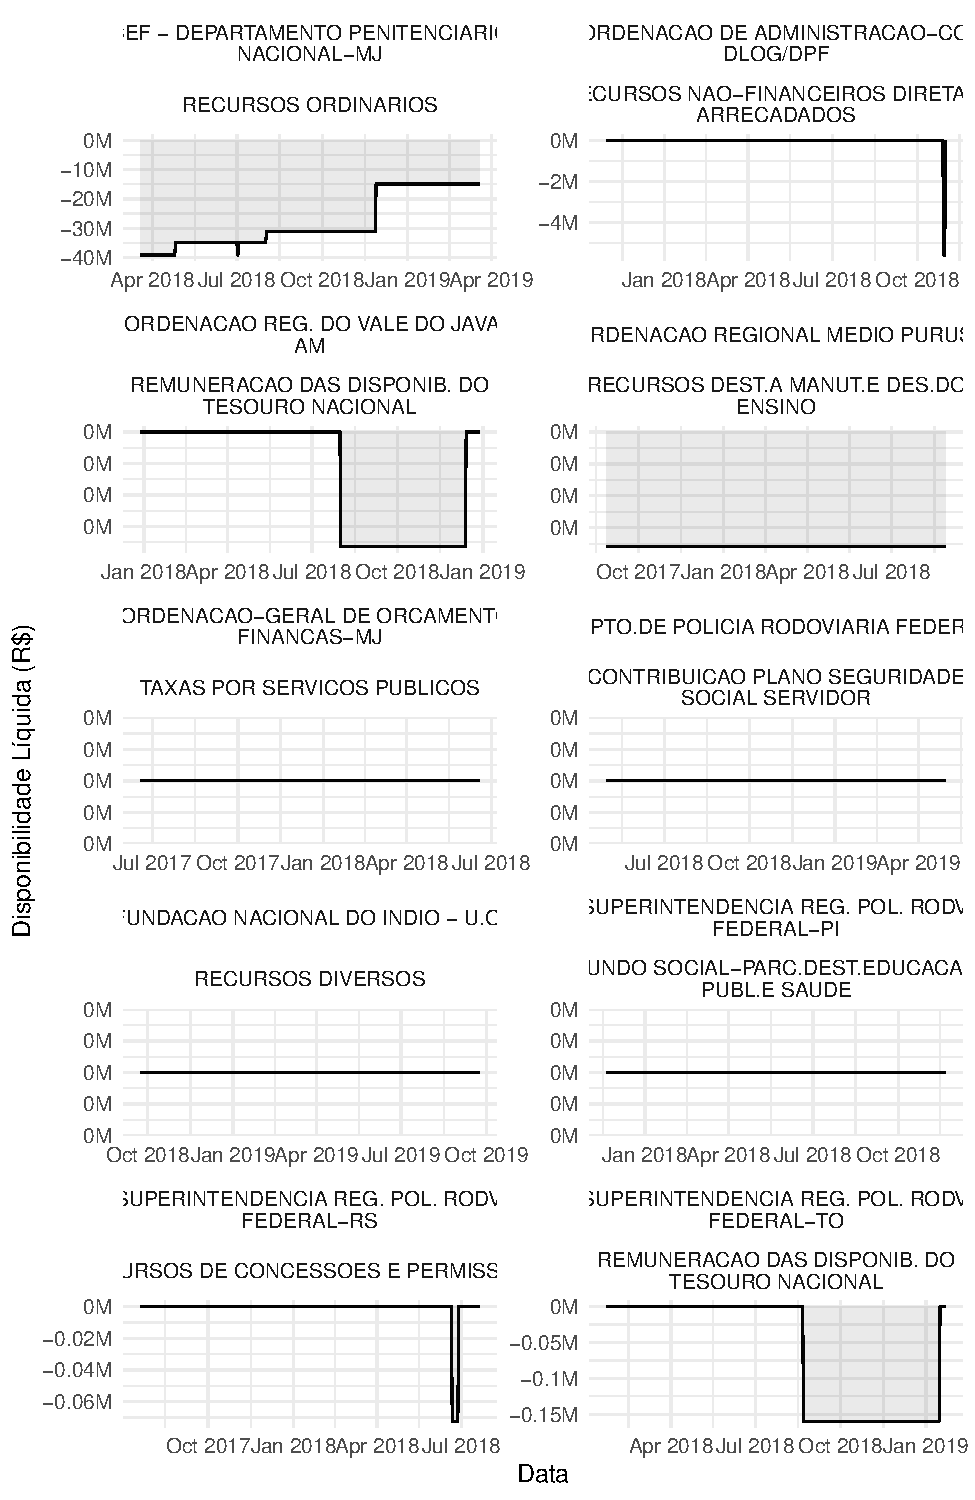
\includegraphics{03-quadro-historico_files/figure-latex/unnamed-chunk-6-1.pdf}

\hypertarget{distribuiuxe7uxe3o-dos-indicadores}{%
\section{Distribuição dos indicadores}\label{distribuiuxe7uxe3o-dos-indicadores}}

Vamos analisar a distribuição dos indicadores em alguns níveis.

\hypertarget{ugfonte}{%
\subsection{Ug/Fonte}\label{ugfonte}}

\begin{itemize}
\tightlist
\item
  gráfico de jitter
\item
  alguma descricao em texto do tipo 30\% das UG/Fonte tem valor acima de x que é considerado alto\ldots{}
\item
  histograma
\item
  alguns exemplos de cada faixa
\end{itemize}

\hypertarget{ug}{%
\subsection{UG}\label{ug}}

\begin{itemize}
\tightlist
\item
  gráfico de jitter
\item
  histograma
\item
  alguns exemplos de cada faixa
\end{itemize}

\hypertarget{fonte}{%
\subsection{Fonte}\label{fonte}}

\begin{itemize}
\tightlist
\item
  gráfico de jitter
\item
  histograma
\item
  alguns exemplos de cada faixa
\item
  destacar a fonte `recursos ordinários'
\end{itemize}

\hypertarget{indicador-de-valor-nominal-r}{%
\section{Indicador de Valor Nominal (R\$)}\label{indicador-de-valor-nominal-r}}

O valor nominal indica o montante que a UG possui disponível em caixa. Quanto maior o excedente de caixa de uma UG, maior a tendência ao empoçamento.

\hypertarget{definiuxe7uxe3o-2}{%
\subsection{Definição}\label{definiuxe7uxe3o-2}}

O indicador de valor nominal no mês \(t\) é definido simplesmente pela disponibilidade líquida no fim do período.

\[IVN_t = DisponibilidadeLíquida_t\]
\#\#\# Exemplos

\hypertarget{distribuiuxe7uxe3o}{%
\subsection{Distribuição}\label{distribuiuxe7uxe3o}}

\hypertarget{indicador-de-disponibilidade-luxedquida-projetada-por-12-meses}{%
\section{Indicador de disponibilidade líquida projetada por 12 meses}\label{indicador-de-disponibilidade-luxedquida-projetada-por-12-meses}}

A disponibilidade líquida mostra o caixa atual de uma UG considerando os pagamentos que foram aprovados até aquele mês (mesmo que ainda não tenham sido realizados). Para ser mais conservador consideramos neste índice os pagamentos que seriam aprovados até os próximos 12 meses - assim sendo, uma UG que ternha valores positivos neste indicador tinha no momento \(t\) um excedente de caixa maior do que o que ela precisaria nos próximos 12 meses.

\hypertarget{definiuxe7uxe3o-3}{%
\subsection{Definição}\label{definiuxe7uxe3o-3}}

O indicador é definido da seguinte maneira:

\[IDL_{12m} = DisponibilidadeBruta_t - \sum_{i=t}^{t+12}Pagamentos_i\]

\hypertarget{exemplos-2}{%
\subsection{Exemplos}\label{exemplos-2}}

\hypertarget{distribuiuxe7uxe3o-1}{%
\subsection{Distribuição}\label{distribuiuxe7uxe3o-1}}

\hypertarget{indicador-de-tempo}{%
\section{Indicador de Tempo}\label{indicador-de-tempo}}

Este indicador considera o tempo que uma UG permanece com disponibilidade líquida positiva. Quando uma UG permanece por muito tempo com disponibilidade positiva isso pode indicar que existe \emph{empoçamento}.

\hypertarget{definiuxe7uxe3o-4}{%
\subsection{Definição}\label{definiuxe7uxe3o-4}}

O indicador é definido por:

\[IT = \sum I(DisponibilidadeLíquida_t > 0)\]

\hypertarget{exemplos-3}{%
\subsection{Exemplos}\label{exemplos-3}}

\hypertarget{distribuiuxe7uxe3o-2}{%
\subsection{Distribuição}\label{distribuiuxe7uxe3o-2}}

\hypertarget{indicador-de-variauxe7uxe3o-da-disponibilidade-luxedquida}{%
\section{Indicador de Variação da Disponibilidade Líquida}\label{indicador-de-variauxe7uxe3o-da-disponibilidade-luxedquida}}

A taxa de variação da Disponibilidade Líquida com relação ao mesmo período do ano anterior tem como objetivo encontrar UG's que tiveram aumento no excedente de caixa, podendo indicar que existe \emph{empoçamento}.

\hypertarget{definiuxe7uxe3o-5}{%
\subsection{Definição}\label{definiuxe7uxe3o-5}}

O indicador é definido por:

\[IVDL_t = \prod_{i=1}^{12}(1 + T_i)^{1/12}\]

Em que:

\[T_i = \frac{DisponibilidadeLíquida_i}{DisponibilidadeLíquida_{i-12}}\]

\hypertarget{exemplos-4}{%
\subsection{Exemplos}\label{exemplos-4}}

\hypertarget{distribuiuxe7uxe3o-3}{%
\subsection{Distribuição}\label{distribuiuxe7uxe3o-3}}

\hypertarget{quadro-analuxedtico-preditivo}{%
\chapter{Quadro analítico preditivo}\label{quadro-analuxedtico-preditivo}}

\hypertarget{fontes-de-recursos-que-tendem-a-acumular-recurso}{%
\section{Fontes de recursos que tendem a acumular recurso}\label{fontes-de-recursos-que-tendem-a-acumular-recurso}}

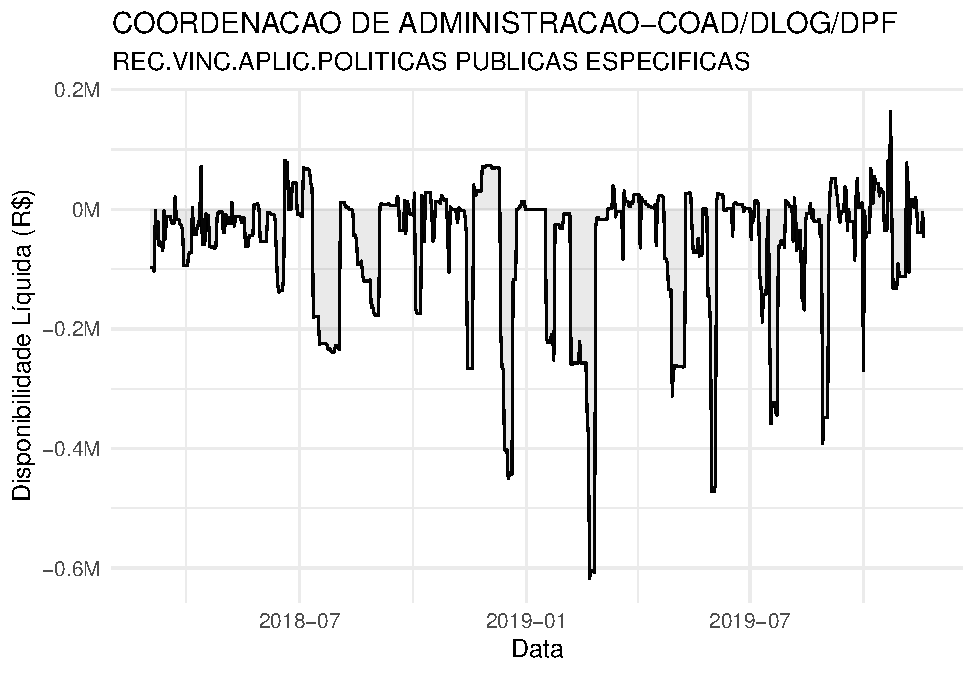
\includegraphics{04-quadro-preditivo_files/figure-latex/unnamed-chunk-2-1.pdf}

A tendência é que as fontes de recursos

\begin{itemize}
\tightlist
\item
  \textbf{destinados às atividades com fins de seguridade social},
\item
  \textbf{não financeiros diretamente arrecadados} e
\item
  \textbf{ordinários}
\end{itemize}

tenham perfil recursos de acumulantes enquanto que as fontes de recursos

\begin{itemize}
\tightlist
\item
  \textbf{de consessões e permissões},
  -\textbf{livres da seguridade social},
\item
  \textbf{fundo social parcialmente destinados à educação pública e saúde},
\item
  \textbf{destinados a manutenção e desenvolvimento do ensino} e
\item
  \textbf{de alienação de bens e direito do patrimônio público}
\end{itemize}

tendem a não acumularem.

\hypertarget{previsuxe3o-de-disponibilidade-luxedquida}{%
\section{Previsão de disponibilidade líquida}\label{previsuxe3o-de-disponibilidade-luxedquida}}

Construímos modelos de séries temporais para previsão de disponibilidade líquida para cada fonte de recursos e UGs.
O desempenho dos modelos foi avaliado para os períodos de 1 semana, 1 mês, 6 meses e 1 ano.

Foi construída uma calculadora em Shiny para consultar as previsões e resultados de cada um dos cenários.

\hypertarget{referuxeancias}{%
\chapter*{Referências}\label{referuxeancias}}
\addcontentsline{toc}{chapter}{Referências}

\begin{itemize}
\tightlist
\item
  NatGep migration waves
\end{itemize}

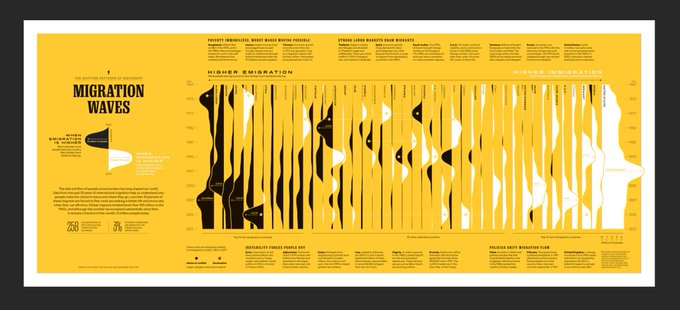
\includegraphics{natgeo.jpg}

\url{https://twitter.com/aLucasLopez/status/1153646875427385344?s=20}

\begin{itemize}
\item
  \href{https://vallandingham.me/bubble_charts_with_d3v4.html}{Diagrama de bolhas em D3 do Jim Vallandingham}.
\item
  \url{https://www.nature.com/articles/s41598-017-13448-3}
\item
  \url{https://github.com/gm-spacagna/deep-ttf/}
\end{itemize}

\backmatter
  \bibliography{book.bib,packages.bib}

\end{document}
